% Created by tikzDevice version 0.7.0 on 2014-10-27 14:13:01
% !TEX encoding = UTF-8 Unicode
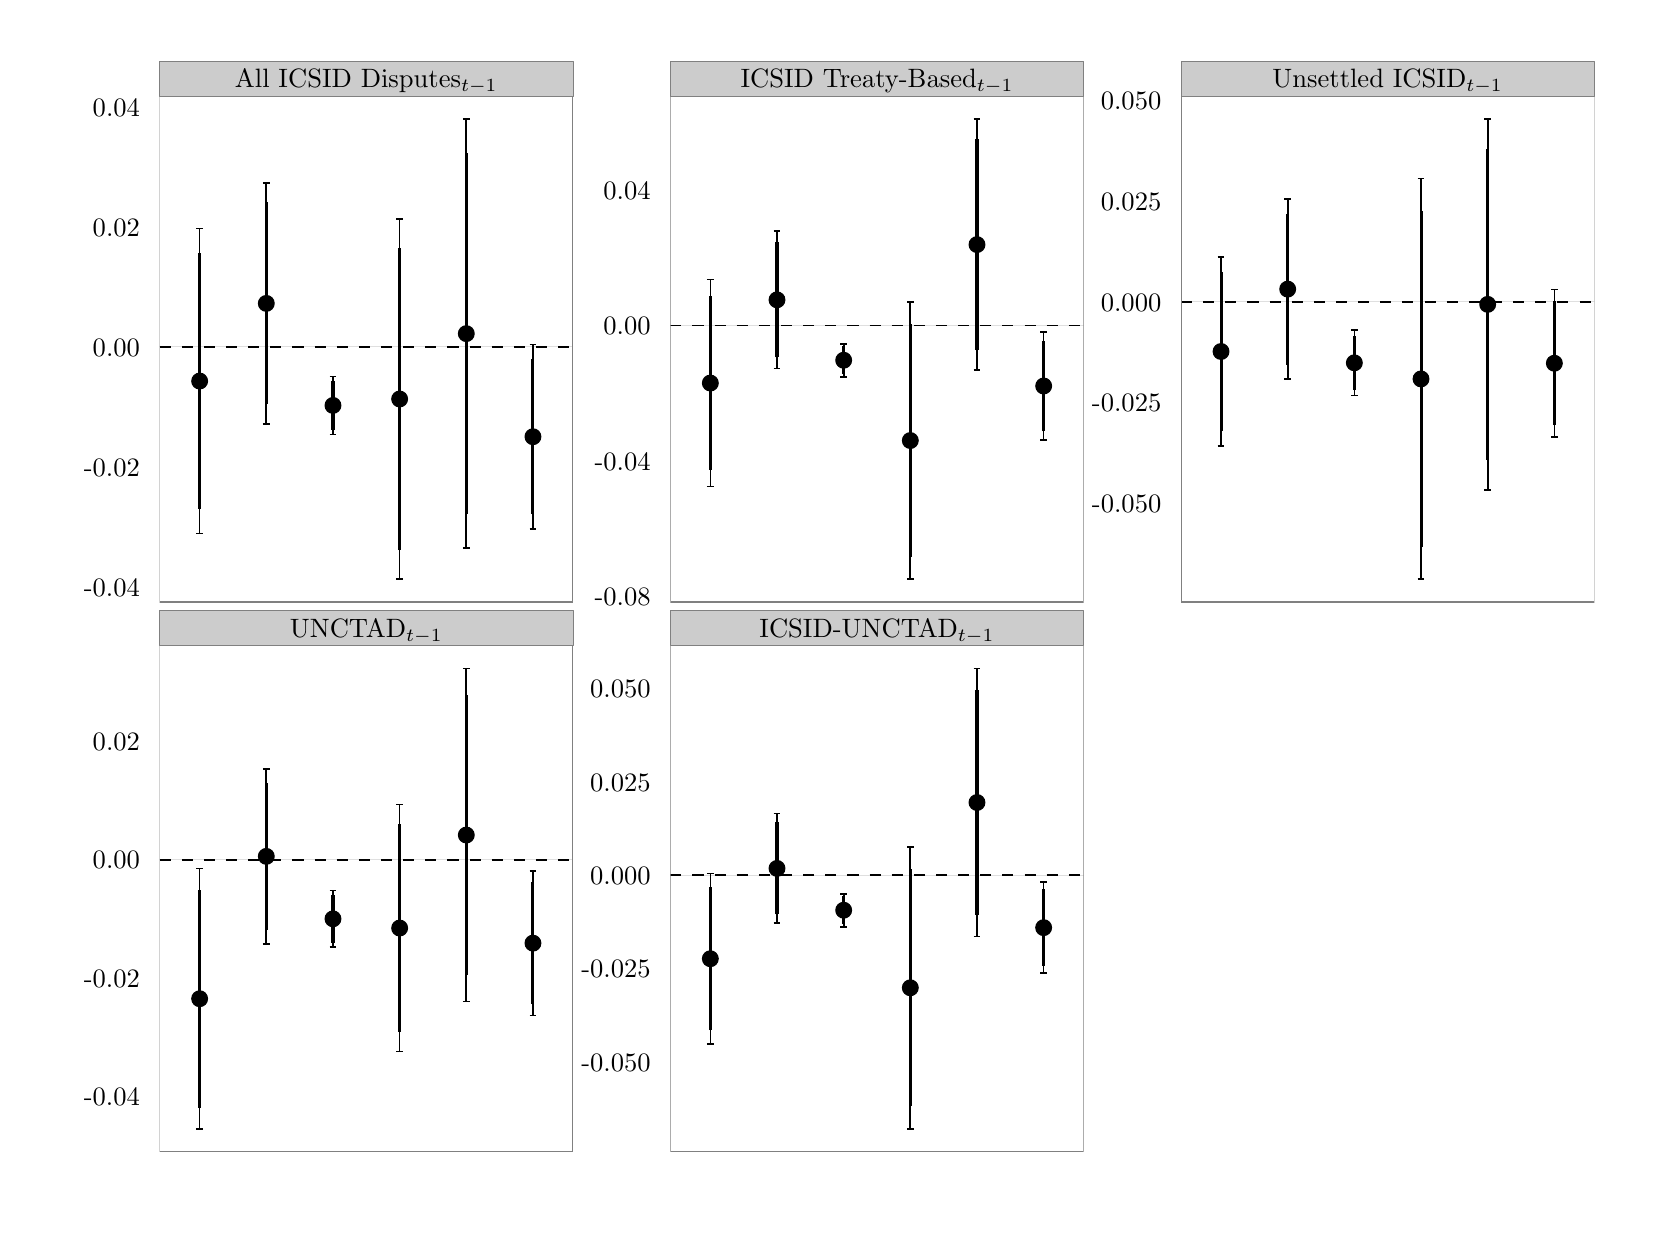
\begin{tikzpicture}[x=1pt,y=1pt]
\definecolor[named]{fillColor}{rgb}{1.00,1.00,1.00}
\path[use as bounding box,fill=fillColor,fill opacity=0.00] (0,0) rectangle (578.16,433.62);
\begin{scope}
\path[clip] (  0.00,  0.00) rectangle (578.16,433.62);
\definecolor[named]{drawColor}{rgb}{1.00,1.00,1.00}
\definecolor[named]{fillColor}{rgb}{1.00,1.00,1.00}

\path[draw=drawColor,line width= 0.6pt,line join=round,line cap=round,fill=fillColor] (  0.00,  0.00) rectangle (578.16,433.62);
\end{scope}
\begin{scope}
\path[clip] ( 47.68,226.00) rectangle (197.04,408.94);
\definecolor[named]{fillColor}{rgb}{1.00,1.00,1.00}

\path[fill=fillColor] ( 47.68,226.00) rectangle (197.04,408.94);
\definecolor[named]{drawColor}{rgb}{0.00,0.00,0.00}
\definecolor[named]{fillColor}{rgb}{0.00,0.00,0.00}

\path[draw=drawColor,draw opacity=0.30,line width= 0.3pt,line join=round,fill=fillColor,fill opacity=0.30] ( 62.14,250.85) -- ( 62.14,361.00);

\path[draw=drawColor,draw opacity=0.30,line width= 0.3pt,line join=round,fill=fillColor,fill opacity=0.30] ( 86.23,290.49) -- ( 86.23,377.47);

\path[draw=drawColor,draw opacity=0.30,line width= 0.3pt,line join=round,fill=fillColor,fill opacity=0.30] (110.32,286.67) -- (110.32,307.56);

\path[draw=drawColor,draw opacity=0.30,line width= 0.3pt,line join=round,fill=fillColor,fill opacity=0.30] (134.41,234.32) -- (134.41,364.56);

\path[draw=drawColor,draw opacity=0.30,line width= 0.3pt,line join=round,fill=fillColor,fill opacity=0.30] (158.50,245.50) -- (158.50,400.63);

\path[draw=drawColor,draw opacity=0.30,line width= 0.3pt,line join=round,fill=fillColor,fill opacity=0.30] (182.58,252.55) -- (182.58,319.07);
\definecolor[named]{drawColor}{rgb}{0.00,0.00,0.00}
\definecolor[named]{fillColor}{rgb}{0.00,0.00,0.00}

\path[draw=drawColor,line width= 1.1pt,line join=round,fill=fillColor] ( 62.14,259.70) -- ( 62.14,352.14);

\path[draw=drawColor,line width= 1.1pt,line join=round,fill=fillColor] ( 86.23,297.48) -- ( 86.23,370.48);

\path[draw=drawColor,line width= 1.1pt,line join=round,fill=fillColor] (110.32,288.35) -- (110.32,305.88);

\path[draw=drawColor,line width= 1.1pt,line join=round,fill=fillColor] (134.41,244.79) -- (134.41,354.09);

\path[draw=drawColor,line width= 1.1pt,line join=round,fill=fillColor] (158.50,257.97) -- (158.50,388.16);

\path[draw=drawColor,line width= 1.1pt,line join=round,fill=fillColor] (182.58,257.90) -- (182.58,313.73);

\path[draw=drawColor,line width= 0.6pt,dash pattern=on 4pt off 4pt ,line join=round,fill=fillColor] ( 47.68,318.26) -- (197.04,318.26);

\path[draw=drawColor,line width= 0.4pt,line join=round,line cap=round,fill=fillColor] ( 62.14,305.92) circle (  2.85);

\path[draw=drawColor,line width= 0.4pt,line join=round,line cap=round,fill=fillColor] ( 86.23,333.98) circle (  2.85);

\path[draw=drawColor,line width= 0.4pt,line join=round,line cap=round,fill=fillColor] (110.32,297.11) circle (  2.85);

\path[draw=drawColor,line width= 0.4pt,line join=round,line cap=round,fill=fillColor] (134.41,299.44) circle (  2.85);

\path[draw=drawColor,line width= 0.4pt,line join=round,line cap=round,fill=fillColor] (158.50,323.06) circle (  2.85);

\path[draw=drawColor,line width= 0.4pt,line join=round,line cap=round,fill=fillColor] (182.58,285.81) circle (  2.85);

\path[draw=drawColor,line width= 0.6pt,line join=round] ( 60.93,361.00) --
	( 63.34,361.00);

\path[draw=drawColor,line width= 0.6pt,line join=round] ( 62.14,361.00) --
	( 62.14,250.85);

\path[draw=drawColor,line width= 0.6pt,line join=round] ( 60.93,250.85) --
	( 63.34,250.85);

\path[draw=drawColor,line width= 0.6pt,line join=round] ( 85.02,377.47) --
	( 87.43,377.47);

\path[draw=drawColor,line width= 0.6pt,line join=round] ( 86.23,377.47) --
	( 86.23,290.49);

\path[draw=drawColor,line width= 0.6pt,line join=round] ( 85.02,290.49) --
	( 87.43,290.49);

\path[draw=drawColor,line width= 0.6pt,line join=round] (109.11,307.56) --
	(111.52,307.56);

\path[draw=drawColor,line width= 0.6pt,line join=round] (110.32,307.56) --
	(110.32,286.67);

\path[draw=drawColor,line width= 0.6pt,line join=round] (109.11,286.67) --
	(111.52,286.67);

\path[draw=drawColor,line width= 0.6pt,line join=round] (133.20,364.56) --
	(135.61,364.56);

\path[draw=drawColor,line width= 0.6pt,line join=round] (134.41,364.56) --
	(134.41,234.32);

\path[draw=drawColor,line width= 0.6pt,line join=round] (133.20,234.32) --
	(135.61,234.32);

\path[draw=drawColor,line width= 0.6pt,line join=round] (157.29,400.63) --
	(159.70,400.63);

\path[draw=drawColor,line width= 0.6pt,line join=round] (158.50,400.63) --
	(158.50,245.50);

\path[draw=drawColor,line width= 0.6pt,line join=round] (157.29,245.50) --
	(159.70,245.50);

\path[draw=drawColor,line width= 0.6pt,line join=round] (181.38,319.07) --
	(183.79,319.07);

\path[draw=drawColor,line width= 0.6pt,line join=round] (182.58,319.07) --
	(182.58,252.55);

\path[draw=drawColor,line width= 0.6pt,line join=round] (181.38,252.55) --
	(183.79,252.55);
\definecolor[named]{drawColor}{rgb}{0.50,0.50,0.50}

\path[draw=drawColor,line width= 0.6pt,line join=round,line cap=round] ( 47.68,226.00) rectangle (197.04,408.94);
\end{scope}
\begin{scope}
\path[clip] (232.22,226.00) rectangle (381.58,408.94);
\definecolor[named]{fillColor}{rgb}{1.00,1.00,1.00}

\path[fill=fillColor] (232.22,226.00) rectangle (381.58,408.94);
\definecolor[named]{drawColor}{rgb}{0.00,0.00,0.00}
\definecolor[named]{fillColor}{rgb}{0.00,0.00,0.00}

\path[draw=drawColor,draw opacity=0.30,line width= 0.3pt,line join=round,fill=fillColor,fill opacity=0.30] (246.68,267.78) -- (246.68,342.62);

\path[draw=drawColor,draw opacity=0.30,line width= 0.3pt,line join=round,fill=fillColor,fill opacity=0.30] (270.77,310.46) -- (270.77,360.08);

\path[draw=drawColor,draw opacity=0.30,line width= 0.3pt,line join=round,fill=fillColor,fill opacity=0.30] (294.86,307.45) -- (294.86,319.43);

\path[draw=drawColor,draw opacity=0.30,line width= 0.3pt,line join=round,fill=fillColor,fill opacity=0.30] (318.94,234.32) -- (318.94,334.51);

\path[draw=drawColor,draw opacity=0.30,line width= 0.3pt,line join=round,fill=fillColor,fill opacity=0.30] (343.03,309.84) -- (343.03,400.63);

\path[draw=drawColor,draw opacity=0.30,line width= 0.3pt,line join=round,fill=fillColor,fill opacity=0.30] (367.12,284.59) -- (367.12,323.70);
\definecolor[named]{drawColor}{rgb}{0.00,0.00,0.00}
\definecolor[named]{fillColor}{rgb}{0.00,0.00,0.00}

\path[draw=drawColor,line width= 1.1pt,line join=round,fill=fillColor] (246.68,273.80) -- (246.68,336.60);

\path[draw=drawColor,line width= 1.1pt,line join=round,fill=fillColor] (270.77,314.45) -- (270.77,356.10);

\path[draw=drawColor,line width= 1.1pt,line join=round,fill=fillColor] (294.86,308.41) -- (294.86,318.47);

\path[draw=drawColor,line width= 1.1pt,line join=round,fill=fillColor] (318.94,242.37) -- (318.94,326.46);

\path[draw=drawColor,line width= 1.1pt,line join=round,fill=fillColor] (343.03,317.14) -- (343.03,393.33);

\path[draw=drawColor,line width= 1.1pt,line join=round,fill=fillColor] (367.12,287.73) -- (367.12,320.56);

\path[draw=drawColor,line width= 0.6pt,dash pattern=on 4pt off 4pt ,line join=round,fill=fillColor] (232.22,326.00) -- (381.58,326.00);

\path[draw=drawColor,line width= 0.4pt,line join=round,line cap=round,fill=fillColor] (246.68,305.20) circle (  2.85);

\path[draw=drawColor,line width= 0.4pt,line join=round,line cap=round,fill=fillColor] (270.77,335.27) circle (  2.85);

\path[draw=drawColor,line width= 0.4pt,line join=round,line cap=round,fill=fillColor] (294.86,313.44) circle (  2.85);

\path[draw=drawColor,line width= 0.4pt,line join=round,line cap=round,fill=fillColor] (318.94,284.42) circle (  2.85);

\path[draw=drawColor,line width= 0.4pt,line join=round,line cap=round,fill=fillColor] (343.03,355.23) circle (  2.85);

\path[draw=drawColor,line width= 0.4pt,line join=round,line cap=round,fill=fillColor] (367.12,304.14) circle (  2.85);

\path[draw=drawColor,line width= 0.6pt,line join=round] (245.47,342.62) --
	(247.88,342.62);

\path[draw=drawColor,line width= 0.6pt,line join=round] (246.68,342.62) --
	(246.68,267.78);

\path[draw=drawColor,line width= 0.6pt,line join=round] (245.47,267.78) --
	(247.88,267.78);

\path[draw=drawColor,line width= 0.6pt,line join=round] (269.56,360.08) --
	(271.97,360.08);

\path[draw=drawColor,line width= 0.6pt,line join=round] (270.77,360.08) --
	(270.77,310.46);

\path[draw=drawColor,line width= 0.6pt,line join=round] (269.56,310.46) --
	(271.97,310.46);

\path[draw=drawColor,line width= 0.6pt,line join=round] (293.65,319.43) --
	(296.06,319.43);

\path[draw=drawColor,line width= 0.6pt,line join=round] (294.86,319.43) --
	(294.86,307.45);

\path[draw=drawColor,line width= 0.6pt,line join=round] (293.65,307.45) --
	(296.06,307.45);

\path[draw=drawColor,line width= 0.6pt,line join=round] (317.74,334.51) --
	(320.15,334.51);

\path[draw=drawColor,line width= 0.6pt,line join=round] (318.94,334.51) --
	(318.94,234.32);

\path[draw=drawColor,line width= 0.6pt,line join=round] (317.74,234.32) --
	(320.15,234.32);

\path[draw=drawColor,line width= 0.6pt,line join=round] (341.83,400.63) --
	(344.24,400.63);

\path[draw=drawColor,line width= 0.6pt,line join=round] (343.03,400.63) --
	(343.03,309.84);

\path[draw=drawColor,line width= 0.6pt,line join=round] (341.83,309.84) --
	(344.24,309.84);

\path[draw=drawColor,line width= 0.6pt,line join=round] (365.92,323.70) --
	(368.33,323.70);

\path[draw=drawColor,line width= 0.6pt,line join=round] (367.12,323.70) --
	(367.12,284.59);

\path[draw=drawColor,line width= 0.6pt,line join=round] (365.92,284.59) --
	(368.33,284.59);
\definecolor[named]{drawColor}{rgb}{0.50,0.50,0.50}

\path[draw=drawColor,line width= 0.6pt,line join=round,line cap=round] (232.22,226.00) rectangle (381.58,408.94);
\end{scope}
\begin{scope}
\path[clip] (416.76,226.00) rectangle (566.12,408.94);
\definecolor[named]{fillColor}{rgb}{1.00,1.00,1.00}

\path[fill=fillColor] (416.76,226.00) rectangle (566.12,408.94);
\definecolor[named]{drawColor}{rgb}{0.00,0.00,0.00}
\definecolor[named]{fillColor}{rgb}{0.00,0.00,0.00}

\path[draw=drawColor,draw opacity=0.30,line width= 0.3pt,line join=round,fill=fillColor,fill opacity=0.30] (431.22,282.54) -- (431.22,350.65);

\path[draw=drawColor,draw opacity=0.30,line width= 0.3pt,line join=round,fill=fillColor,fill opacity=0.30] (455.30,306.59) -- (455.30,371.69);

\path[draw=drawColor,draw opacity=0.30,line width= 0.3pt,line join=round,fill=fillColor,fill opacity=0.30] (479.39,300.75) -- (479.39,324.27);

\path[draw=drawColor,draw opacity=0.30,line width= 0.3pt,line join=round,fill=fillColor,fill opacity=0.30] (503.48,234.32) -- (503.48,379.06);

\path[draw=drawColor,draw opacity=0.30,line width= 0.3pt,line join=round,fill=fillColor,fill opacity=0.30] (527.57,266.64) -- (527.57,400.63);

\path[draw=drawColor,draw opacity=0.30,line width= 0.3pt,line join=round,fill=fillColor,fill opacity=0.30] (551.66,285.67) -- (551.66,339.05);
\definecolor[named]{drawColor}{rgb}{0.00,0.00,0.00}
\definecolor[named]{fillColor}{rgb}{0.00,0.00,0.00}

\path[draw=drawColor,line width= 1.1pt,line join=round,fill=fillColor] (431.22,288.02) -- (431.22,345.18);

\path[draw=drawColor,line width= 1.1pt,line join=round,fill=fillColor] (455.30,311.82) -- (455.30,366.46);

\path[draw=drawColor,line width= 1.1pt,line join=round,fill=fillColor] (479.39,302.64) -- (479.39,322.37);

\path[draw=drawColor,line width= 1.1pt,line join=round,fill=fillColor] (503.48,245.95) -- (503.48,367.42);

\path[draw=drawColor,line width= 1.1pt,line join=round,fill=fillColor] (527.57,277.41) -- (527.57,389.85);

\path[draw=drawColor,line width= 1.1pt,line join=round,fill=fillColor] (551.66,289.96) -- (551.66,334.75);

\path[draw=drawColor,line width= 0.6pt,dash pattern=on 4pt off 4pt ,line join=round,fill=fillColor] (416.76,334.50) -- (566.12,334.50);

\path[draw=drawColor,line width= 0.4pt,line join=round,line cap=round,fill=fillColor] (431.22,316.60) circle (  2.85);

\path[draw=drawColor,line width= 0.4pt,line join=round,line cap=round,fill=fillColor] (455.30,339.14) circle (  2.85);

\path[draw=drawColor,line width= 0.4pt,line join=round,line cap=round,fill=fillColor] (479.39,312.51) circle (  2.85);

\path[draw=drawColor,line width= 0.4pt,line join=round,line cap=round,fill=fillColor] (503.48,306.69) circle (  2.85);

\path[draw=drawColor,line width= 0.4pt,line join=round,line cap=round,fill=fillColor] (527.57,333.63) circle (  2.85);

\path[draw=drawColor,line width= 0.4pt,line join=round,line cap=round,fill=fillColor] (551.66,312.36) circle (  2.85);

\path[draw=drawColor,line width= 0.6pt,line join=round] (430.01,350.65) --
	(432.42,350.65);

\path[draw=drawColor,line width= 0.6pt,line join=round] (431.22,350.65) --
	(431.22,282.54);

\path[draw=drawColor,line width= 0.6pt,line join=round] (430.01,282.54) --
	(432.42,282.54);

\path[draw=drawColor,line width= 0.6pt,line join=round] (454.10,371.69) --
	(456.51,371.69);

\path[draw=drawColor,line width= 0.6pt,line join=round] (455.30,371.69) --
	(455.30,306.59);

\path[draw=drawColor,line width= 0.6pt,line join=round] (454.10,306.59) --
	(456.51,306.59);

\path[draw=drawColor,line width= 0.6pt,line join=round] (478.19,324.27) --
	(480.60,324.27);

\path[draw=drawColor,line width= 0.6pt,line join=round] (479.39,324.27) --
	(479.39,300.75);

\path[draw=drawColor,line width= 0.6pt,line join=round] (478.19,300.75) --
	(480.60,300.75);

\path[draw=drawColor,line width= 0.6pt,line join=round] (502.28,379.06) --
	(504.69,379.06);

\path[draw=drawColor,line width= 0.6pt,line join=round] (503.48,379.06) --
	(503.48,234.32);

\path[draw=drawColor,line width= 0.6pt,line join=round] (502.28,234.32) --
	(504.69,234.32);

\path[draw=drawColor,line width= 0.6pt,line join=round] (526.37,400.63) --
	(528.78,400.63);

\path[draw=drawColor,line width= 0.6pt,line join=round] (527.57,400.63) --
	(527.57,266.64);

\path[draw=drawColor,line width= 0.6pt,line join=round] (526.37,266.64) --
	(528.78,266.64);

\path[draw=drawColor,line width= 0.6pt,line join=round] (550.46,339.05) --
	(552.87,339.05);

\path[draw=drawColor,line width= 0.6pt,line join=round] (551.66,339.05) --
	(551.66,285.67);

\path[draw=drawColor,line width= 0.6pt,line join=round] (550.46,285.67) --
	(552.87,285.67);
\definecolor[named]{drawColor}{rgb}{0.50,0.50,0.50}

\path[draw=drawColor,line width= 0.6pt,line join=round,line cap=round] (416.76,226.00) rectangle (566.12,408.94);
\end{scope}
\begin{scope}
\path[clip] ( 47.68, 27.42) rectangle (197.04,210.36);
\definecolor[named]{fillColor}{rgb}{1.00,1.00,1.00}

\path[fill=fillColor] ( 47.68, 27.42) rectangle (197.04,210.36);
\definecolor[named]{drawColor}{rgb}{0.00,0.00,0.00}
\definecolor[named]{fillColor}{rgb}{0.00,0.00,0.00}

\path[draw=drawColor,draw opacity=0.30,line width= 0.3pt,line join=round,fill=fillColor,fill opacity=0.30] ( 62.14, 35.74) -- ( 62.14,129.73);

\path[draw=drawColor,draw opacity=0.30,line width= 0.3pt,line join=round,fill=fillColor,fill opacity=0.30] ( 86.23,102.50) -- ( 86.23,165.83);

\path[draw=drawColor,draw opacity=0.30,line width= 0.3pt,line join=round,fill=fillColor,fill opacity=0.30] (110.32,101.33) -- (110.32,121.87);

\path[draw=drawColor,draw opacity=0.30,line width= 0.3pt,line join=round,fill=fillColor,fill opacity=0.30] (134.41, 63.67) -- (134.41,152.87);

\path[draw=drawColor,draw opacity=0.30,line width= 0.3pt,line join=round,fill=fillColor,fill opacity=0.30] (158.50, 81.69) -- (158.50,202.04);

\path[draw=drawColor,draw opacity=0.30,line width= 0.3pt,line join=round,fill=fillColor,fill opacity=0.30] (182.58, 76.71) -- (182.58,128.92);
\definecolor[named]{drawColor}{rgb}{0.00,0.00,0.00}
\definecolor[named]{fillColor}{rgb}{0.00,0.00,0.00}

\path[draw=drawColor,line width= 1.1pt,line join=round,fill=fillColor] ( 62.14, 43.29) -- ( 62.14,122.17);

\path[draw=drawColor,line width= 1.1pt,line join=round,fill=fillColor] ( 86.23,107.59) -- ( 86.23,160.74);

\path[draw=drawColor,line width= 1.1pt,line join=round,fill=fillColor] (110.32,102.98) -- (110.32,120.22);

\path[draw=drawColor,line width= 1.1pt,line join=round,fill=fillColor] (134.41, 70.84) -- (134.41,145.70);

\path[draw=drawColor,line width= 1.1pt,line join=round,fill=fillColor] (158.50, 91.37) -- (158.50,192.37);

\path[draw=drawColor,line width= 1.1pt,line join=round,fill=fillColor] (182.58, 80.90) -- (182.58,124.73);

\path[draw=drawColor,line width= 0.6pt,dash pattern=on 4pt off 4pt ,line join=round,fill=fillColor] ( 47.68,132.95) -- (197.04,132.95);

\path[draw=drawColor,line width= 0.4pt,line join=round,line cap=round,fill=fillColor] ( 62.14, 82.73) circle (  2.85);

\path[draw=drawColor,line width= 0.4pt,line join=round,line cap=round,fill=fillColor] ( 86.23,134.17) circle (  2.85);

\path[draw=drawColor,line width= 0.4pt,line join=round,line cap=round,fill=fillColor] (110.32,111.60) circle (  2.85);

\path[draw=drawColor,line width= 0.4pt,line join=round,line cap=round,fill=fillColor] (134.41,108.27) circle (  2.85);

\path[draw=drawColor,line width= 0.4pt,line join=round,line cap=round,fill=fillColor] (158.50,141.87) circle (  2.85);

\path[draw=drawColor,line width= 0.4pt,line join=round,line cap=round,fill=fillColor] (182.58,102.81) circle (  2.85);

\path[draw=drawColor,line width= 0.6pt,line join=round] ( 60.93,129.73) --
	( 63.34,129.73);

\path[draw=drawColor,line width= 0.6pt,line join=round] ( 62.14,129.73) --
	( 62.14, 35.74);

\path[draw=drawColor,line width= 0.6pt,line join=round] ( 60.93, 35.74) --
	( 63.34, 35.74);

\path[draw=drawColor,line width= 0.6pt,line join=round] ( 85.02,165.83) --
	( 87.43,165.83);

\path[draw=drawColor,line width= 0.6pt,line join=round] ( 86.23,165.83) --
	( 86.23,102.50);

\path[draw=drawColor,line width= 0.6pt,line join=round] ( 85.02,102.50) --
	( 87.43,102.50);

\path[draw=drawColor,line width= 0.6pt,line join=round] (109.11,121.87) --
	(111.52,121.87);

\path[draw=drawColor,line width= 0.6pt,line join=round] (110.32,121.87) --
	(110.32,101.33);

\path[draw=drawColor,line width= 0.6pt,line join=round] (109.11,101.33) --
	(111.52,101.33);

\path[draw=drawColor,line width= 0.6pt,line join=round] (133.20,152.87) --
	(135.61,152.87);

\path[draw=drawColor,line width= 0.6pt,line join=round] (134.41,152.87) --
	(134.41, 63.67);

\path[draw=drawColor,line width= 0.6pt,line join=round] (133.20, 63.67) --
	(135.61, 63.67);

\path[draw=drawColor,line width= 0.6pt,line join=round] (157.29,202.04) --
	(159.70,202.04);

\path[draw=drawColor,line width= 0.6pt,line join=round] (158.50,202.04) --
	(158.50, 81.69);

\path[draw=drawColor,line width= 0.6pt,line join=round] (157.29, 81.69) --
	(159.70, 81.69);

\path[draw=drawColor,line width= 0.6pt,line join=round] (181.38,128.92) --
	(183.79,128.92);

\path[draw=drawColor,line width= 0.6pt,line join=round] (182.58,128.92) --
	(182.58, 76.71);

\path[draw=drawColor,line width= 0.6pt,line join=round] (181.38, 76.71) --
	(183.79, 76.71);
\definecolor[named]{drawColor}{rgb}{0.50,0.50,0.50}

\path[draw=drawColor,line width= 0.6pt,line join=round,line cap=round] ( 47.68, 27.42) rectangle (197.04,210.36);
\end{scope}
\begin{scope}
\path[clip] (232.22, 27.42) rectangle (381.58,210.36);
\definecolor[named]{fillColor}{rgb}{1.00,1.00,1.00}

\path[fill=fillColor] (232.22, 27.42) rectangle (381.58,210.36);
\definecolor[named]{drawColor}{rgb}{0.00,0.00,0.00}
\definecolor[named]{fillColor}{rgb}{0.00,0.00,0.00}

\path[draw=drawColor,draw opacity=0.30,line width= 0.3pt,line join=round,fill=fillColor,fill opacity=0.30] (246.68, 66.40) -- (246.68,127.96);

\path[draw=drawColor,draw opacity=0.30,line width= 0.3pt,line join=round,fill=fillColor,fill opacity=0.30] (270.77,110.00) -- (270.77,149.65);

\path[draw=drawColor,draw opacity=0.30,line width= 0.3pt,line join=round,fill=fillColor,fill opacity=0.30] (294.86,108.76) -- (294.86,120.67);

\path[draw=drawColor,draw opacity=0.30,line width= 0.3pt,line join=round,fill=fillColor,fill opacity=0.30] (318.94, 35.74) -- (318.94,137.62);

\path[draw=drawColor,draw opacity=0.30,line width= 0.3pt,line join=round,fill=fillColor,fill opacity=0.30] (343.03,105.21) -- (343.03,202.04);

\path[draw=drawColor,draw opacity=0.30,line width= 0.3pt,line join=round,fill=fillColor,fill opacity=0.30] (367.12, 91.98) -- (367.12,124.84);
\definecolor[named]{drawColor}{rgb}{0.00,0.00,0.00}
\definecolor[named]{fillColor}{rgb}{0.00,0.00,0.00}

\path[draw=drawColor,line width= 1.1pt,line join=round,fill=fillColor] (246.68, 71.35) -- (246.68,123.01);

\path[draw=drawColor,line width= 1.1pt,line join=round,fill=fillColor] (270.77,113.19) -- (270.77,146.46);

\path[draw=drawColor,line width= 1.1pt,line join=round,fill=fillColor] (294.86,109.71) -- (294.86,119.71);

\path[draw=drawColor,line width= 1.1pt,line join=round,fill=fillColor] (318.94, 43.93) -- (318.94,129.43);

\path[draw=drawColor,line width= 1.1pt,line join=round,fill=fillColor] (343.03,113.00) -- (343.03,194.26);

\path[draw=drawColor,line width= 1.1pt,line join=round,fill=fillColor] (367.12, 94.62) -- (367.12,122.20);

\path[draw=drawColor,line width= 0.6pt,dash pattern=on 4pt off 4pt ,line join=round,fill=fillColor] (232.22,127.33) -- (381.58,127.33);

\path[draw=drawColor,line width= 0.4pt,line join=round,line cap=round,fill=fillColor] (246.68, 97.18) circle (  2.85);

\path[draw=drawColor,line width= 0.4pt,line join=round,line cap=round,fill=fillColor] (270.77,129.82) circle (  2.85);

\path[draw=drawColor,line width= 0.4pt,line join=round,line cap=round,fill=fillColor] (294.86,114.71) circle (  2.85);

\path[draw=drawColor,line width= 0.4pt,line join=round,line cap=round,fill=fillColor] (318.94, 86.68) circle (  2.85);

\path[draw=drawColor,line width= 0.4pt,line join=round,line cap=round,fill=fillColor] (343.03,153.63) circle (  2.85);

\path[draw=drawColor,line width= 0.4pt,line join=round,line cap=round,fill=fillColor] (367.12,108.41) circle (  2.85);

\path[draw=drawColor,line width= 0.6pt,line join=round] (245.47,127.96) --
	(247.88,127.96);

\path[draw=drawColor,line width= 0.6pt,line join=round] (246.68,127.96) --
	(246.68, 66.40);

\path[draw=drawColor,line width= 0.6pt,line join=round] (245.47, 66.40) --
	(247.88, 66.40);

\path[draw=drawColor,line width= 0.6pt,line join=round] (269.56,149.65) --
	(271.97,149.65);

\path[draw=drawColor,line width= 0.6pt,line join=round] (270.77,149.65) --
	(270.77,110.00);

\path[draw=drawColor,line width= 0.6pt,line join=round] (269.56,110.00) --
	(271.97,110.00);

\path[draw=drawColor,line width= 0.6pt,line join=round] (293.65,120.67) --
	(296.06,120.67);

\path[draw=drawColor,line width= 0.6pt,line join=round] (294.86,120.67) --
	(294.86,108.76);

\path[draw=drawColor,line width= 0.6pt,line join=round] (293.65,108.76) --
	(296.06,108.76);

\path[draw=drawColor,line width= 0.6pt,line join=round] (317.74,137.62) --
	(320.15,137.62);

\path[draw=drawColor,line width= 0.6pt,line join=round] (318.94,137.62) --
	(318.94, 35.74);

\path[draw=drawColor,line width= 0.6pt,line join=round] (317.74, 35.74) --
	(320.15, 35.74);

\path[draw=drawColor,line width= 0.6pt,line join=round] (341.83,202.04) --
	(344.24,202.04);

\path[draw=drawColor,line width= 0.6pt,line join=round] (343.03,202.04) --
	(343.03,105.21);

\path[draw=drawColor,line width= 0.6pt,line join=round] (341.83,105.21) --
	(344.24,105.21);

\path[draw=drawColor,line width= 0.6pt,line join=round] (365.92,124.84) --
	(368.33,124.84);

\path[draw=drawColor,line width= 0.6pt,line join=round] (367.12,124.84) --
	(367.12, 91.98);

\path[draw=drawColor,line width= 0.6pt,line join=round] (365.92, 91.98) --
	(368.33, 91.98);
\definecolor[named]{drawColor}{rgb}{0.50,0.50,0.50}

\path[draw=drawColor,line width= 0.6pt,line join=round,line cap=round] (232.22, 27.42) rectangle (381.58,210.36);
\end{scope}
\begin{scope}
\path[clip] (  0.00,  0.00) rectangle (578.16,433.62);
\definecolor[named]{drawColor}{rgb}{0.50,0.50,0.50}
\definecolor[named]{fillColor}{rgb}{0.80,0.80,0.80}

\path[draw=drawColor,line width= 0.2pt,line join=round,line cap=round,fill=fillColor] ( 47.68,408.94) rectangle (197.04,421.57);
\definecolor[named]{drawColor}{rgb}{0.00,0.00,0.00}

\node[text=drawColor,anchor=base,inner sep=0pt, outer sep=0pt, scale=  0.96] at (122.36,411.95) {All ICSID Disputes$_{t-1}$};
\end{scope}
\begin{scope}
\path[clip] (  0.00,  0.00) rectangle (578.16,433.62);
\definecolor[named]{drawColor}{rgb}{0.50,0.50,0.50}
\definecolor[named]{fillColor}{rgb}{0.80,0.80,0.80}

\path[draw=drawColor,line width= 0.2pt,line join=round,line cap=round,fill=fillColor] (232.22,408.94) rectangle (381.58,421.57);
\definecolor[named]{drawColor}{rgb}{0.00,0.00,0.00}

\node[text=drawColor,anchor=base,inner sep=0pt, outer sep=0pt, scale=  0.96] at (306.90,411.95) {ICSID Treaty-Based$_{t-1}$};
\end{scope}
\begin{scope}
\path[clip] (  0.00,  0.00) rectangle (578.16,433.62);
\definecolor[named]{drawColor}{rgb}{0.50,0.50,0.50}
\definecolor[named]{fillColor}{rgb}{0.80,0.80,0.80}

\path[draw=drawColor,line width= 0.2pt,line join=round,line cap=round,fill=fillColor] (416.76,408.94) rectangle (566.12,421.57);
\definecolor[named]{drawColor}{rgb}{0.00,0.00,0.00}

\node[text=drawColor,anchor=base,inner sep=0pt, outer sep=0pt, scale=  0.96] at (491.44,411.95) {Unsettled ICSID$_{t-1}$};
\end{scope}
\begin{scope}
\path[clip] (  0.00,  0.00) rectangle (578.16,433.62);
\definecolor[named]{drawColor}{rgb}{0.50,0.50,0.50}
\definecolor[named]{fillColor}{rgb}{0.80,0.80,0.80}

\path[draw=drawColor,line width= 0.2pt,line join=round,line cap=round,fill=fillColor] ( 47.68,210.36) rectangle (197.04,222.99);
\definecolor[named]{drawColor}{rgb}{0.00,0.00,0.00}

\node[text=drawColor,anchor=base,inner sep=0pt, outer sep=0pt, scale=  0.96] at (122.36,213.37) {UNCTAD$_{t-1}$};
\end{scope}
\begin{scope}
\path[clip] (  0.00,  0.00) rectangle (578.16,433.62);
\definecolor[named]{drawColor}{rgb}{0.50,0.50,0.50}
\definecolor[named]{fillColor}{rgb}{0.80,0.80,0.80}

\path[draw=drawColor,line width= 0.2pt,line join=round,line cap=round,fill=fillColor] (232.22,210.36) rectangle (381.58,222.99);
\definecolor[named]{drawColor}{rgb}{0.00,0.00,0.00}

\node[text=drawColor,anchor=base,inner sep=0pt, outer sep=0pt, scale=  0.96] at (306.90,213.37) {ICSID-UNCTAD$_{t-1}$};
\end{scope}
\begin{scope}
\path[clip] (  0.00,  0.00) rectangle (578.16,433.62);
\definecolor[named]{drawColor}{rgb}{0.00,0.00,0.00}

\node[text=drawColor,anchor=base east,inner sep=0pt, outer sep=0pt, scale=  0.96] at ( 40.57,228.20) {-0.04};

\node[text=drawColor,anchor=base east,inner sep=0pt, outer sep=0pt, scale=  0.96] at ( 40.57,271.57) {-0.02};

\node[text=drawColor,anchor=base east,inner sep=0pt, outer sep=0pt, scale=  0.96] at ( 40.57,314.95) {0.00};

\node[text=drawColor,anchor=base east,inner sep=0pt, outer sep=0pt, scale=  0.96] at ( 40.57,358.33) {0.02};

\node[text=drawColor,anchor=base east,inner sep=0pt, outer sep=0pt, scale=  0.96] at ( 40.57,401.70) {0.04};
\end{scope}
\begin{scope}
\path[clip] (  0.00,  0.00) rectangle (578.16,433.62);
\definecolor[named]{drawColor}{rgb}{0.00,0.00,0.00}

\node[text=drawColor,anchor=base east,inner sep=0pt, outer sep=0pt, scale=  0.96] at (225.11,224.76) {-0.08};

\node[text=drawColor,anchor=base east,inner sep=0pt, outer sep=0pt, scale=  0.96] at (225.11,273.73) {-0.04};

\node[text=drawColor,anchor=base east,inner sep=0pt, outer sep=0pt, scale=  0.96] at (225.11,322.69) {0.00};

\node[text=drawColor,anchor=base east,inner sep=0pt, outer sep=0pt, scale=  0.96] at (225.11,371.66) {0.04};
\end{scope}
\begin{scope}
\path[clip] (  0.00,  0.00) rectangle (578.16,433.62);
\definecolor[named]{drawColor}{rgb}{0.00,0.00,0.00}

\node[text=drawColor,anchor=base east,inner sep=0pt, outer sep=0pt, scale=  0.96] at (409.65,258.35) {-0.050};

\node[text=drawColor,anchor=base east,inner sep=0pt, outer sep=0pt, scale=  0.96] at (409.65,294.78) {-0.025};

\node[text=drawColor,anchor=base east,inner sep=0pt, outer sep=0pt, scale=  0.96] at (409.65,331.20) {0.000};

\node[text=drawColor,anchor=base east,inner sep=0pt, outer sep=0pt, scale=  0.96] at (409.65,367.62) {0.025};

\node[text=drawColor,anchor=base east,inner sep=0pt, outer sep=0pt, scale=  0.96] at (409.65,404.04) {0.050};
\end{scope}
\begin{scope}
\path[clip] (  0.00,  0.00) rectangle (578.16,433.62);
\definecolor[named]{drawColor}{rgb}{0.00,0.00,0.00}

\node[text=drawColor,anchor=base east,inner sep=0pt, outer sep=0pt, scale=  0.96] at ( 40.57, 44.27) {-0.04};

\node[text=drawColor,anchor=base east,inner sep=0pt, outer sep=0pt, scale=  0.96] at ( 40.57, 86.96) {-0.02};

\node[text=drawColor,anchor=base east,inner sep=0pt, outer sep=0pt, scale=  0.96] at ( 40.57,129.64) {0.00};

\node[text=drawColor,anchor=base east,inner sep=0pt, outer sep=0pt, scale=  0.96] at ( 40.57,172.32) {0.02};
\end{scope}
\begin{scope}
\path[clip] (  0.00,  0.00) rectangle (578.16,433.62);
\definecolor[named]{drawColor}{rgb}{0.00,0.00,0.00}

\node[text=drawColor,anchor=base east,inner sep=0pt, outer sep=0pt, scale=  0.96] at (225.11, 56.54) {-0.050};

\node[text=drawColor,anchor=base east,inner sep=0pt, outer sep=0pt, scale=  0.96] at (225.11, 90.29) {-0.025};

\node[text=drawColor,anchor=base east,inner sep=0pt, outer sep=0pt, scale=  0.96] at (225.11,124.03) {0.000};

\node[text=drawColor,anchor=base east,inner sep=0pt, outer sep=0pt, scale=  0.96] at (225.11,157.77) {0.025};

\node[text=drawColor,anchor=base east,inner sep=0pt, outer sep=0pt, scale=  0.96] at (225.11,191.51) {0.050};
\end{scope}
\end{tikzpicture}
